\section{Induktorn}
\textbf{HAREC a.\ref{HAREC.a.2.3}\label{myHAREC.a.2.3}}
\index{induktor}

\subsection{Allmänt}

När elektrisk ström flyter genom en ledare, så alstras ett magnetfält omkring
den. Så snart strömmens styrka eller riktning ändras, uppstår en motsvarande
s.k. elektromotorisk kraft (EMK), som motverkar ändringen. Kraften finns i
magnetfältet, som är lagrad magnetisk energi.


\subsection{Självinduktion - induktans}
\textbf{HAREC a.\ref{HAREC.a.2.3.1}\label{myHAREC.a.2.3.1}}
\index{induktans}

Magnetfältets förmåga att alstra en motverkande EMK kallas självinduktion eller
induktans. Ordet induktans kommer från latinets inducere, som betyder införa.

När en ledare, som ingår i en sluten krets, rör sig i ett magnetfält, så kommer
en ström att flyta genom ledaren på grund av den EMK (spänning) som alstras.
Varje ändring av strömmen motverkas av det magnetfält som strömmen själv
alstrar.

När det uppstår självinduktion i en ledare, så kallas ledaren induktor.
Självinduktionen är jämnt utbredd över ledarens hela längd. När ett större
induktansvärde behövs på något särskilt ställe i strömkretsen, så kan ledarens
längd ökas just där och lindas upp till en spole med lämplig form.
Hela spolen kallas då för induktor.

Det att ett motverkande magnetiskt fält alstras omkring en ledare när strömmen i
den ändras, påverkar kretsens egenskaper och därmed utformning på olika sätt.
Vid snabba strömändringar, t.ex. vid hög frekvens, är motverkan större än vid
långsamma ändringar. Vid konstant likström uppstår däremot ingen motverkan -
självinduktion.

Induktansen är efter resistansen och kapacitansen den vanligaste egenskapen i
en strömkrets.

\subsection{Försök med induktion}

\emph{Försök 1}

\begin{figure}
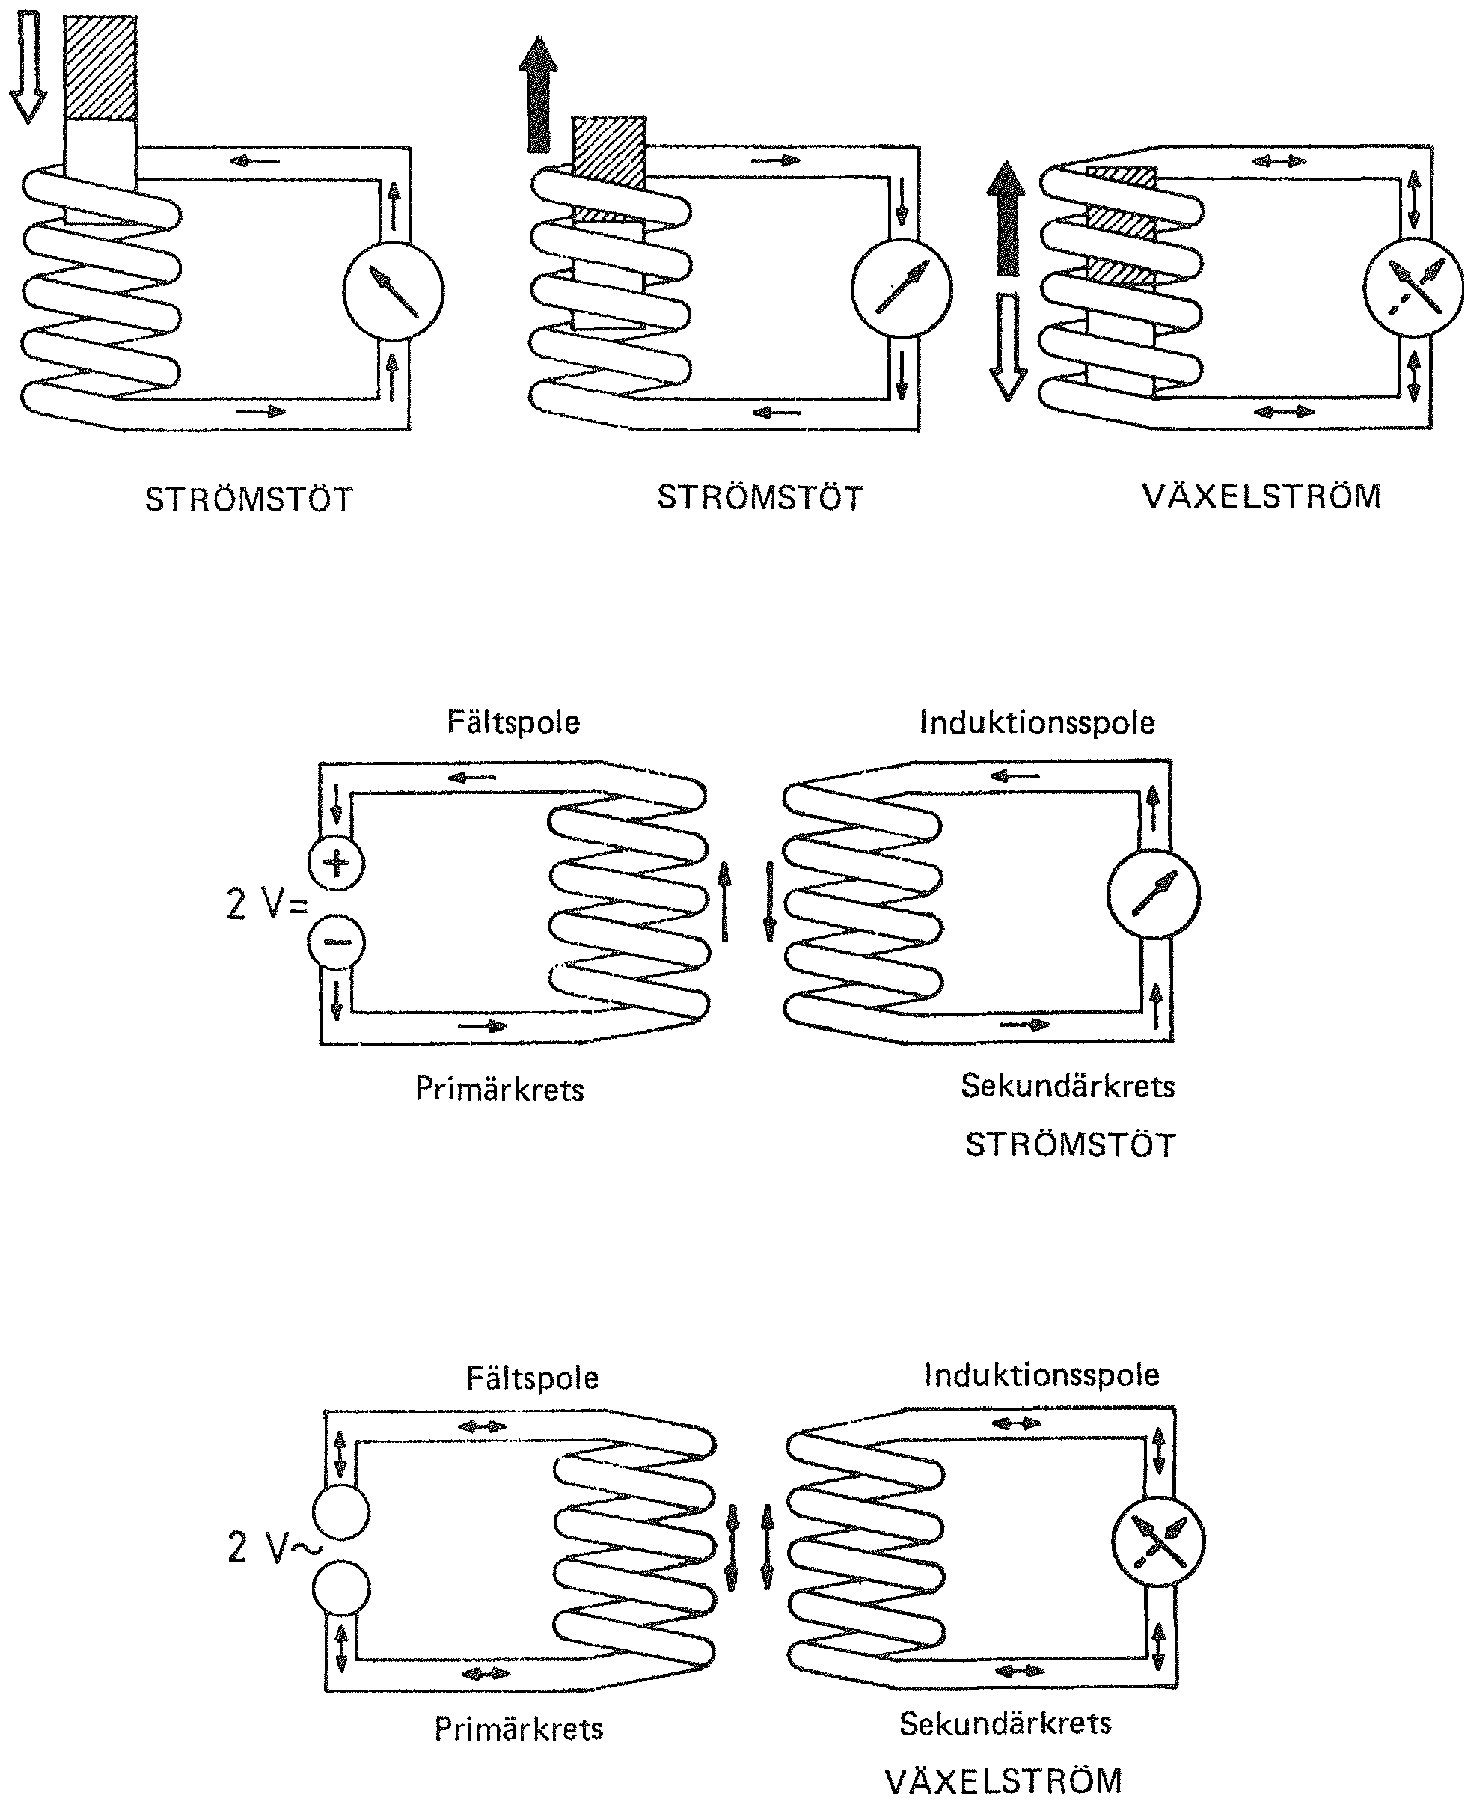
\includegraphics[width=\textwidth]{images/bild_2_2-03}
\caption{Schemasymboler för kondensatorer}
\label{fig:BildII2-3}
\end{figure}

Bild \ref{fig:BildII2-3} överst

Ett känsligt vridspoleinstrument kopplas till en induktor. Instrumentet bör ha
noll på skalans mitt, så att strömriktningen syns. En permanentmagnet används
för att visa att självinduktion uppstår när magneten förs fram och tillbaka
genom induktorn.

Instrumentet ger utslag när magneten är i rörelse. Utslaget blir större vid
snabbare hastighetsändring. Utslagsriktningen växlar, när magneten förs in i
respektive dras ut ur induktorn - det uppstår en växelström.

En växelspänning uppstår över induktorn, även när den ingår i en strömkrets som
sluts och bryts - alltså utan en magnet som rör sig.

\emph{Försök 2}

Bild \ref{fig:BildII2-3} mitten

Permanentmagneten byts nu mot ännu en induktor. Utöver den första induktorn, som
vi nu kallar sekundärlindning, kallar vi den nya induktorn för primärlindning.

När vi släpper ström genom primärlindningen så alstrar den ett magnetfält. Först
är strömmen noll för att sedan \emph{ändras} till ett högt värde och därefter
återgå till noll. Det blir en strömstöt.

Varje ändring alstrar en mot-emk, som bygger upp ett magnetfält, först i en
riktning och sedan i den andra. I båda fallen passerar fältet genom båda
lindningarna. Fältet från primärlindningen inducerar en spänningsstöt i
sekundärlindningen. Stöten har en riktning, när primärlindningens strömkrets
sluts och motsatt riktning när den bryts, d.v.s. det blir en växelspänning.
När sekundärlindningen ingår i en sluten krets, uppstår en växelström genom
sekundärlindningen.

\emph{Försök 3}


Bild \ref{fig:BildII2-3} nederst

Vad händer när primärlindningen i försök 2 ansluts till en växelspänning, t.ex.
med nätfrekvensen 50 Hz? Använd för säkerhets skull en skyddstransformator
mellan nätet och lindningen!

I sekundärlindningen uppstår då spänningsstötar, vars polaritet i detta fall
växlar 100 gånger per sekund. Det uppstår alltså en växelspänning över
sekundärlindningen och om denna ingår i en sluten strömkrets uppstår det en
motsvarande växelström.


\begin{figure}
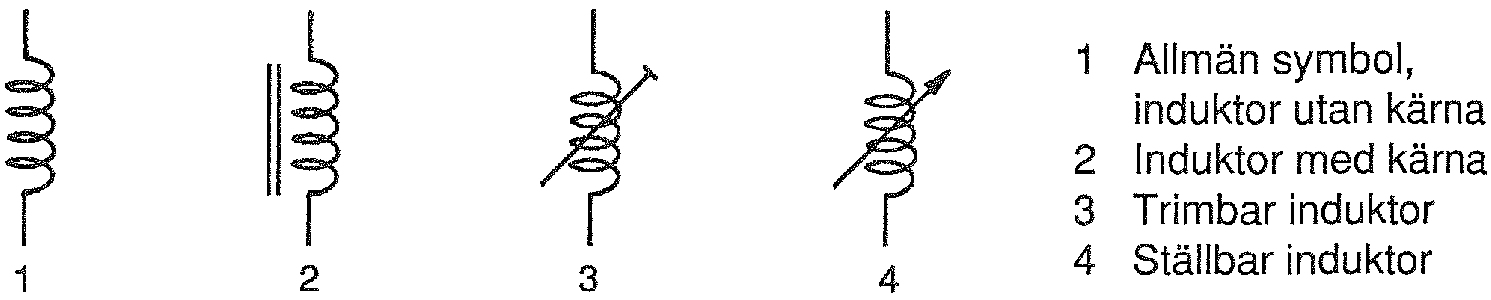
\includegraphics[width=\textwidth]{images/bild_2_2-04}
\caption{Schemasymboler för induktorer}
\label{fig:BildII2-4}
\end{figure}

Bild \ref{fig:BildII2-4}

\subsection{Olika utföranden}

Elektromagneter, drosslar, induktorer för svängningskretsar, ramantenner o.s.v.

\subsection{Enheten Henry (H)}
\textbf{HAREC a.\ref{HAREC.a.2.3.2}\label{myHAREC.a.2.3.2}}
\index{Henry (H)}
\index{enheter!Henry (H)}

Måttenheten för självinduktion är Henry (H). 1 Henry (1 H) är självinduktionen i
en induktor, som alstrar en motspänning av 1 volt vid en strömändring av 1
ampere under 1 sekund.

I formler betecknas induktans med L.

Sambandet är

\(Volt = Henry \cdot Ampere/sekund\)

1 H är en stor måttenhet. För elektroniktillämpningar används därför ett mer
hanterligt format.

Exempel:

\begin{tabular}{ll}
\(1\ H \) & \(= 1000\ mH\) \\
\(1\ mH\) & \(= 1 \cdot 10^{-3}\ H\) \\
\(1\ mH\) & \(= 1000\ µH\) \\
\(1\ µH\) & \(= 1 \cdot 10^{-3}\ mH = 1 \cdot 10^{-6}\ H \)
\end{tabular}

\subsection{Hur induktansen påverkas}
\textbf{HAREC a.\ref{HAREC.a.2.3.3}\label{myHAREC.a.2.3.3}}

Induktansen beror på induktorns mekaniska dimensioner, antalet lindningsvarv och
materialet i kärnan.

Induktansen i en cylindrisk induktor är proportionell mot tvärsnittsytan, omvänt
proportionell mot längden och proportionell mot kvadraten på lindningsvarvtalet.

Induktansen ökar, om induktorn förses med en kärna av järn och minskar med en
kärna av omagnetisk, ledande metall, t.ex. koppar, mässing eller aluminium.

\subsection{Induktiv reaktans}
\textbf{HAREC a.\ref{HAREC.a.2.3.4}\label{myHAREC.a.2.3.4}}
\index{induktiv reaktans}
\index{reaktans!induktiv}

Till skillnad från när en resistor ansluts till en spänning, så blir
strömökningen i en induktor fördröjd. Orsaken är att en induktor inte bara har
en resistans, vilken ju inte påverkas av strömvariationer, utan har även en
induktiv reaktans \(X_L\). Ordet reaktans kommer från latinets re (åter) agere
(verka).

\emph{Reaktans} - växelströmsmotstånd eller skenbart motstånd - uppträder så
länge som strömmen genom induktorn \emph{ändras}. En induktor gör således också
motstånd mot varje strömändring och detta motstånd ökar med ökande
ändringshastighet.

En fullbordad pendling i en växelström kan ses som ett varv i en cirkel - 360° -
och en fullbordad pendling kallas en period.

En period motsvarar omkretsen i en cirkel med radien r, där omkretsen är
\(2 \cdot π \cdot r\). När strömmen växlar 1 gång/sekund har
pendlingen en frekvens [f] av 1 Hertz [Hz]. Vid 50 växlingar/sekund har
pendlingen en frekvens av 50 Hz o.s.v.

\emph{Induktiva reaktansen \(X_L\)} - växelströmsmotståndet i en induktor - är
en funktion av strömmens s.k. vinkelhastighet \(\omega = 2 \cdot π \cdot f\) och
av storheten av induktansen L.

Den induktiva reaktansen är proportionell mot strömmens frekvens och mot
induktorns induktansvärde. Inga förluster uppstår i en ideal induktor, d.v.s. en
som teoretiskt saknar resistans.

Sambandet är
\(X_L = 2πfL = \omega L\)


% I tabellen nedan gjorde jag om lite från originaltexten, och gjorde enligt
% samma mönster som motsvarande tabell för kondensatorn.
% Dessutom användes enheten mH vilket jag ändrade till µH eftersom det gör
% resonemanget konsekvent med motsvarande för kondensatorn.
% // Hans
% Jag tog bort den undre delen i tabellen både här och vid kondensatorn då de
% var felaktiga // NTJ

\begin{tabular}{llll}
 \([\Omega]\) & \([Hz]\) & \([H]\)
 \end{tabular}

\emph{Exempel:}
% Samma resonemang här; jag gjorde stilen mer konsekvent med avsnittet om
% kondensatorn. Ingen egentlig ändring av själva sakinnehållet.

1. \(L = 1\ H\) \(f = 50\ Hz\) \(X_L = ?\)

\(X_L = 2πfL = 2π \cdot 50 \cdot 1 = 314\ Ω\)

2. \(L = 1\ H\) \(f = 5\ kHz\) \(X_L = ?\)

\(X_L = 2πfL = 2π \cdot 5 \cdot 10^3 \cdot 1 = 31\, 400\ Ω\)

\subsection{Fasförskjutning mellan spänning och ström i en induktor}
\textbf{HAREC a.\ref{HAREC.a.2.3.5}\label{myHAREC.a.2.3.5}}
\index{induktor!fasförskjutning}

Bild \ref{fig:BildII3-11}.

Med fasförskjutning menas den tidsmässiga förskjutningen mellan ström- och
spänningsförlopp. Strömmen genom en induktor, når inte sitt toppvärde samtidigt
som spänningen över den. Orsaken är växlingarna mellan elektrisk och magnetisk
energi i induktorn.

I en ideal induktor är spänningen fasförskjuten 90° före strömmen. I praktiken
är dock förskjutningen något mindre än 90° på grund av resistansen i induktorn.

\subsection{Q-faktor - godhetstal}
\textbf{HAREC a.\ref{HAREC.a.2.3.6}\label{myHAREC.a.2.3.6}}
\index{Q-faktor!induktor}

Q-faktorn kan avse två olika saker, som inte ska förväxlas. Det är Q-faktorn
för en komponent respektive den för en hel strömkrets.

Q-faktorn för en induktor är kvoten av dess reaktans och serieresistans.

\(Q_\text{komponent} = \dfrac{X_\text{komponent}}{R_\text{komponent}}\)

Q-faktorn för en hel svängningskrets beror däremot på bredden på det
frekvensband som en viss komponentkombination ger. Q-faktorn för en resonant
svängningskrets är därför ett mått på dess selektivitet (se kapitel \ref{Q-faktor}).

Medan Q-faktorn för en ingående komponent påverkar Q-faktorn för en hel krets,
så gäller inte det omvända.

\subsection{Yteffekt - skin-effect}
\index{yteffekt}
\index{skin-effect}

I en ledare av homogent material fördelar sig en likström lika över hela
tvärsnittet. Strömtätheten för en växelström däremot, minskar i ledarens mitt
och ökar i stället vid ytan. Ju högre frekvensen är, desto större är
strömtätheten vid ytan. Fenomenet kallas yteffekt (på engelska
\emph{skin effect}) och uppträder i alla ledare.

Det djup i ledarmaterialet där laddningstätheten sjunkit till 37\% av
värdet vid ytan kallas \emph{skin depth}. För koppar är detta djup c:a 70 mm vid
100 Hz. Vid 1 MHz har djupet minskat till 0,07 mm och vid 100 MHz till
0,0067 mm. På grund av yteffekten är alltså materialet i mitten av homogena
ledare elektriskt mindre verksamt vid höga frekvenser. Resistansen blir alltså
större för växelström än för likström, om ledaren är samma.

Utöver frekvensen påverkas yteffekten av ledarmaterialets elektriska och
magnetiska ledningsförmåga. För att få låg resistans i ledare för högfrekvent
ström är det viktigt att omkretsen är stor och att materialskiktet vid ytan har
hög ledningsförmåga. Det är därför som induktorerna i sändarslutsteg ofta är
försilvrade och består av rör med stor diameter eller av breda band.

\subsection{Temperaturkoefficient}

Liksom med resistorer, så påverkas induktansen av temperaturen. Att sambandet
mellan induktans och temperatur är viktigt, förstås av att
temperaturkoefficienten i den frekvensbestämmande induktorn i en oscillatorkrets
påverkar frekvensstabiliteten.

Eftersom metallen koppar utvidgar sig vid temperaturökning och induktorns
tvärsnittsyta då blir större, så är temperaturkoefficienten vanligen positiv.
Temperaturkoefficienten \(\alpha_L\) anger induktansändringen per grad temperaturändring.

Induktansändringen blir då

\(∆L = \pm \alpha _L \cdot L_k \cdot ∆\vartheta\)

varvid \(L_k\) är induktansvärdet vid den lägre temperaturen (oftast 20 °C) och
\(∆\vartheta\) är temperaturändringen i °Kelvin.

Kelvin [K] är den normerade måttenheten för absolut temperatur. En ändring med
1 K motsvarar en ändring med 1 °C.

Induktorer kan innehålla kärnor av någon metallegering, vars egenskaper också är
temperaturberoende.

I praktiken kan man knappast påverka temperaturkoefficienten i en induktor.
Eftersom en svängningskrets för det mesta även innehåller kondensatorer, så kan
man t.ex. kompensera en positiv temperaturkoefficient i induktorn med en negativ
i en kondensator.

\subsection{Förluster i kärnmaterial}

När ett magnetiskt växelfält passerar ett kärnmaterial så kommer atomerna (som
är permanentmagneter) att ständigt inta nya lägen i materialet i takt med
fältets frekvens. Då uppstår virvelströmmar, s.k. järnförluster, som dels
påverkar materialets ledningsförmåga och dels höjer temperaturen i kärnan och
därmed i hela induktorn.
